\documentclass[aspectratio=169]{beamer}
\usefonttheme{serif}

\usepackage{graphicx}
\usepackage[english]{babel}
\usepackage[T1]{fontenc}
\usepackage{pdfx, csquotes, xcolor, xspace, changepage, setspace}
\usepackage{libertinus}
\usepackage[maxbibnames=99]{biblatex}

\title{Knowledge Refinement in\\Expressive Description Logics}
\author{Roland Bernard}
\date{July 2023}

\definecolor{unibzblue}{HTML}{0086ec}
\definecolor{unibzblue2}{HTML}{edf7ff}

\setbeamercolor{outerbox}{fg=black,bg=unibzblue2}
\setbeamercolor{innerbox}{fg=white,bg=unibzblue}

\setbeamertemplate{title page}{
  \scriptsize 
  \begin{tabular}{ll}
    \multicolumn{2}{r}{
\includegraphics[width=0.3\linewidth]{resources/unibz-logo.png}} \\
    \multicolumn{2}{l}{\raggedright Bachelor Thesis} \\
    \\
    \multicolumn{2}{p{\linewidth}}{\raggedright \huge \bf \inserttitle} \\
    \vspace*{5mm} \\
    Candidate   & \insertauthor \\
    \\
    Supervisors & Oliver Kutz \\
                & Nicolas Troquard \\
    \\
    \multicolumn{2}{p{\linewidth}}{\insertdate}
  \end{tabular}
}

\setbeamertemplate{frametitle}{
  \vspace*{6mm}
  \Large \bf \color{black} \insertframetitle
}

\setbeamertemplate{itemize items}{\scriptsize\raisebox{0.6mm}{\color{unibzblue} $\blacktriangleright$}}

\newcommand{\ALC}{\ensuremath{\texorpdfstring{\mathcal{ALC}}{ALC}}\xspace}
\newcommand{\SROIQ}{\ensuremath{\texorpdfstring{\mathcal{SROIQ}}{SROIQ}}\xspace}
\newcommand{\ALCHOIQ}{\ensuremath{\texorpdfstring{\mathcal{ALCHOIQ}}{ALCHOIQ}}\xspace}
\newcommand{\ALCH}{\ensuremath{\texorpdfstring{\mathcal{ALCH}}{ALCH}}\xspace}

\newcommand{\Lmc}{\ensuremath{\mathcal{L}}\xspace}
\newcommand{\Tmc}{\ensuremath{\mathcal{T}}\xspace}
\newcommand{\Amc}{\ensuremath{\mathcal{A}}\xspace}
\newcommand{\Rmc}{\ensuremath{\mathcal{R}}\xspace}
\newcommand{\Omc}{\ensuremath{\mathcal{O}}\xspace}
\newcommand{\Omcref}{\ensuremath{{\mathcal{O}^\textnormal{ref}}}\xspace}
\newcommand{\Omcfull}{\ensuremath{{\mathcal{O}^\textnormal{full}}}\xspace}

\newcommand{\op}[1]{\operatorname{#1}}
\newcommand{\Inf}{{\ensuremath{\op{Inf}}}\xspace}
\newcommand{\sub}{{\ensuremath{\op{sub}}}\xspace}
\newcommand{\qual}{{\ensuremath{\op{IIC}}}\xspace}
\newcommand{\UpC}{{\ensuremath{\op{UpCover}}}\xspace}
\newcommand{\DownC}{{\ensuremath{\op{DownCover}}}\xspace}
\newcommand{\inv}{\ensuremath{\op{inv}}\xspace}
\newcommand{\refine}{\ensuremath{\op{\uparrow}}\xspace}
\newcommand{\corefine}{\ensuremath{\op{\downarrow}}\xspace}

\newcommand{\disjoint}{\ensuremath{\op{disjoint}}\xspace}
\newcommand{\self}{\ensuremath{\mathit{Self}}\xspace}
\newcommand{\less}[2]{\ensuremath{\leq #1~#2}\xspace}
\newcommand{\more}[2]{\ensuremath{\geq #1~#2}\xspace}
\newcommand{\nominal}[1]{\ensuremath{\{#1\}}\xspace}

\newcommand{\sitem}{{\scriptsize\raisebox{0.2mm}{\color{unibzblue} $\rightarrow$}}\enspace}

\newlength{\offsetpage}
\newenvironment{narrowpage}[1][3mm]{
  \setlength{\offsetpage}{#1}
  \begin{adjustwidth}{\offsetpage}{\offsetpage}
  \addtolength{\textwidth}{-2\offsetpage}
}{\end{adjustwidth}}

\newenvironment{items}{\begin{narrowpage}\vfill}{\end{narrowpage}}
\newenvironment{oitem}[1][2mm]{\hfill\begin{beamercolorbox}[rounded=true,colsep=#1]{outerbox}\parbox[t]{5mm}{\scriptsize\raisebox{0.6mm}{\color{unibzblue} $\blacktriangleright$}}\begin{minipage}[t]{\textwidth}}{\end{minipage}\end{beamercolorbox}\hfill\vfill}

\beamertemplatenavigationsymbolsempty
\setbeamertemplate{footline}{}

\begin{document}

\frame{\titlepage}

\begin{frame}
  \frametitle{Description Logics}
  \begin{items}
    \begin{oitem}[1mm]
      Family of logics used in knowledge representation \\
      \sitem {\footnotesize aiming for favorable trade-offs between complexity and expressivity}
    \end{oitem}
    \begin{oitem}[1mm]
      \begin{tabular}[t]{@{}ll}
        {\footnotesize Individuals, e.g.,} & $\mathit{roland}$ \quad $\mathit{oliver}$ \quad $\mathit{nicolas}$ \quad $\mathit{unibz}$ \quad $\mathit{blue}$ \\
        {\footnotesize Concepts, e.g.,} & $\mathit{Student}$ \quad $\mathit{Professor}$ \quad $\mathit{Person}$ \quad $\mathit{University}$ \quad $\mathit{Color}$ \\
        {\footnotesize Roles, e.g.,} & $\mathit{studiesAt}$ \quad $\mathit{supervisedBy}$ \quad $\mathit{hasColor}$ \\
      \end{tabular}
    \end{oitem}
    \begin{oitem}[1mm]
      \begin{tabular}[t]{@{}ll}
        {\footnotesize Complex concepts, e.g.,} & $\lnot \mathit{Person}$ \quad $\mathit{Person} \sqcap \mathit{Student}$ \quad $\exists studiesAt.University$
      \end{tabular}
    \end{oitem}
    \begin{oitem}[1mm]
      \begin{tabular}[t]{@{}ll}
        {\footnotesize Axioms e.g.,} & $\mathit{Student}(\mathit{roland})$ \quad $\mathit{Student} \sqsubseteq \mathit{Person}$ \quad $\mathit{studiesAt}(roland, unibz)$
      \end{tabular}
    \end{oitem}
  \end{items}
\end{frame}

\begin{frame}
  \frametitle{Expressive \textnormal{Description Logics}}
  \begin{items}
    \begin{oitem}
      Additional kinds of concept expressions and axioms, e.g., \\
      \begin{tabular}[t]{@{}ll}
        \sitem {\footnotesize role inclusions, e.g.,} & $\mathit{motherOf} \sqsubseteq \mathit{parentOf}$ \\
        \sitem {\footnotesize cardinality constraints, e.g.,} & $\less 1 {\mathit{studiesAt}.\mathit{University}}$ \quad $\more 2 {\mathit{supervisedBy}.\top}$ \\
      \end{tabular}
    \end{oitem}
    \begin{oitem}
      Require additional rules to guarantee decidability \\
      \sitem {\footnotesize separation into simple and non-simple roles} \\
      \sitem {\footnotesize limits on the graph formed by role inclusions}
    \end{oitem}
    \begin{oitem}
      Focus on \SROIQ and the Web Ontology Language
    \end{oitem}
  \end{items}
\end{frame}

\begin{frame}
  \frametitle{Knowledge Refinement \textnormal{in Expressive Description Logics}}
% * Process of iteratively mofifying and improving knowleadge
% * Concept refinement
% * Axiom weakening
\end{frame}

\begin{frame}
  \frametitle{Applications of Knowledge Refinement}
% * Repairing ontologies
% * Combination of conflicting knowledge
% * Machine learning
\end{frame}

\begin{frame}
  \frametitle{Challenges in Weakening Expressive Description Logics}
% * simple and non-simple
% * regularity
% * restrictions have been added to prevent problems
\end{frame}

\begin{frame}
  \frametitle{Implementation of Axiom Weakening}
% * implemented iin Java using the OWL API
% * Using highly-optimized of-the-shelf reasoners
% * extensive tests of the main functionality
\end{frame}

\begin{frame}
  \frametitle{A Protégé Plugin supporting these Techniques}
% * manual axiom weakening
% * configurable automatic remairs
\end{frame}

\begin{frame}
  \frametitle{Evaluating Axiom Weakening for Ontology Repair}
% * We want a repair to retain as many consequences as possible
% * For comparing two repairs O1 and O2 define the IIC
\end{frame}

\begin{frame}
  \frametitle{Evaluation Results}
  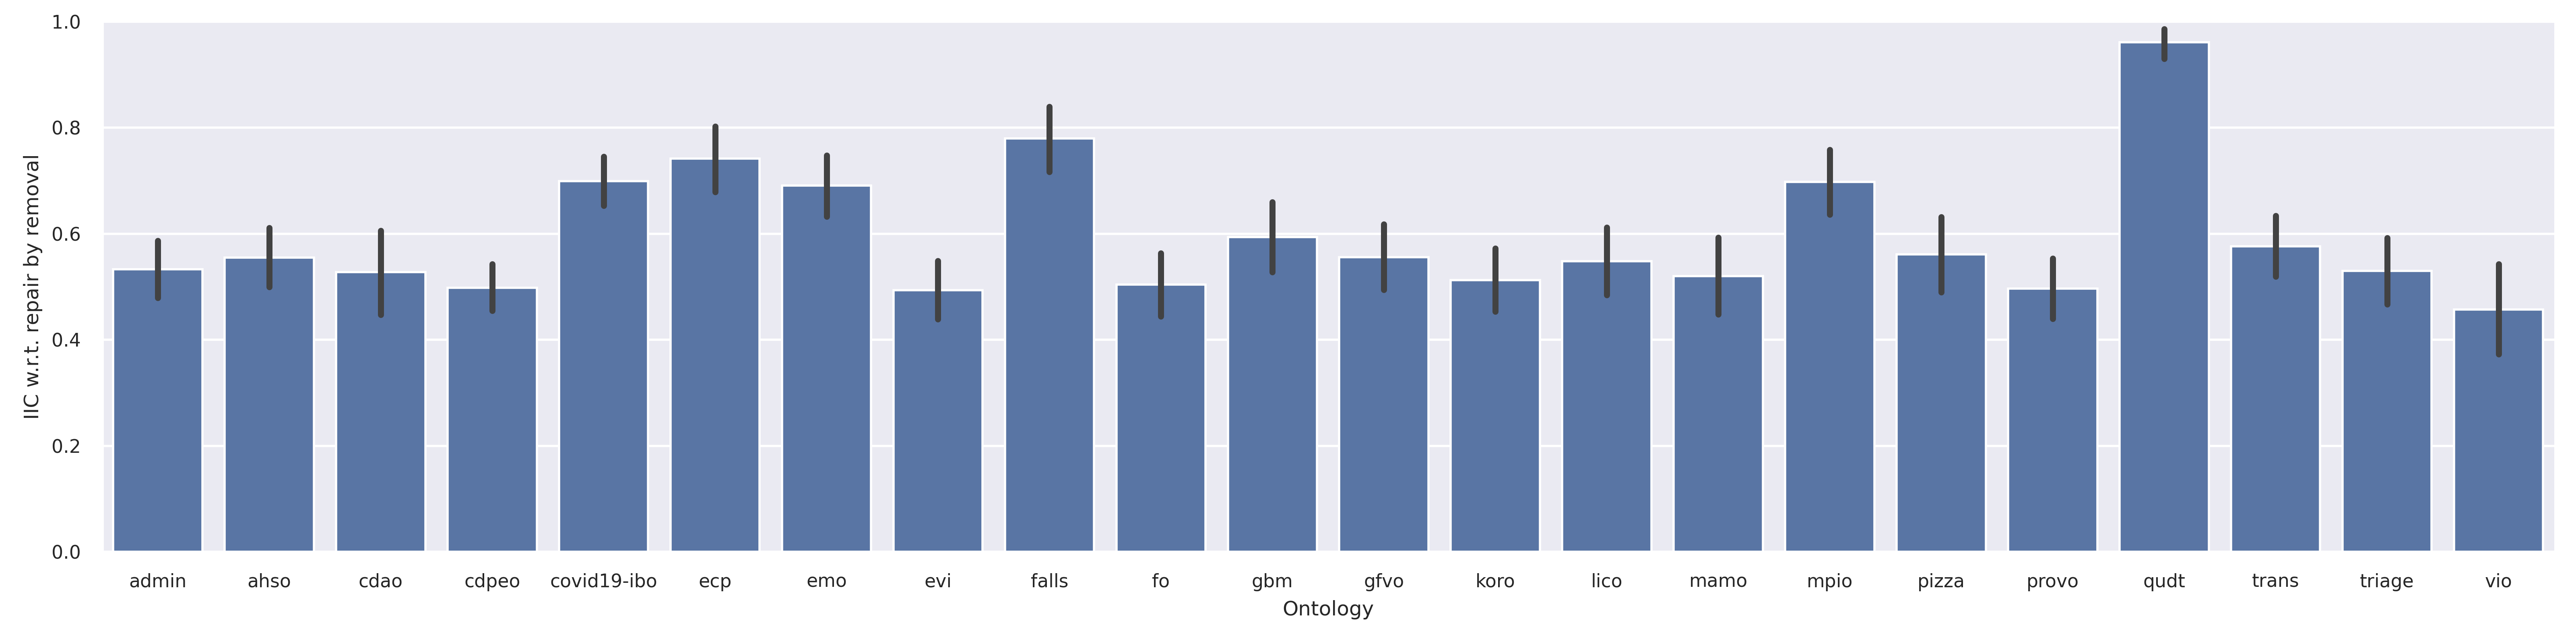
\includegraphics[width=\textwidth]{resources/iic-remove-ontology-bar.png}
\end{frame}

\begin{frame}
  \frametitle{Outcomes of the Thesis}
  \begin{items}
    \begin{oitem}
      Extended the axiom weakening operator to \SROIQ \\
      \sitem {\footnotesize and showed that the proposed approach maintains the necessary constraints}
    \end{oitem}
    \begin{oitem}
      Developed a Protégé plugin for applying these techniques \\
      \sitem {\footnotesize allowing users to easily use the techniques described in the thesis}
    \end{oitem}
    \begin{oitem}
      Evaluated the proposed approach on real-world ontologies \\
      \sitem {\footnotesize showing that axiom weakening can outperform removal}
    \end{oitem}
  \end{items}
\end{frame}

\begin{frame}
  \frametitle{Future Outlook}
% * Loosen the restrictions of the axiom weakening
% * Better ways to guide the repairs
% * Find better measuers to compare repair quality
\end{frame}

{
\setbeamercolor{background canvas}{bg=black}
\begin{frame}[plain]{}
\end{frame}
}

\end{document}
